\chapter{Hand Features and Representations}

Different hand feature representation and encoding methods are compared. The
hand features can be extracted from either color, depth or both images. 
\begin{figure}[h]
  \centering
  \subfigure[Color images] {
	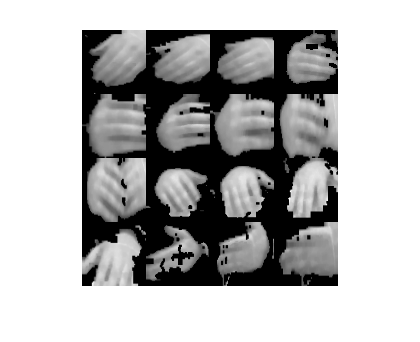
\includegraphics[width=0.45\textwidth]{figures/color_hand.png} 
  }
  \subfigure[Depth images] {
  	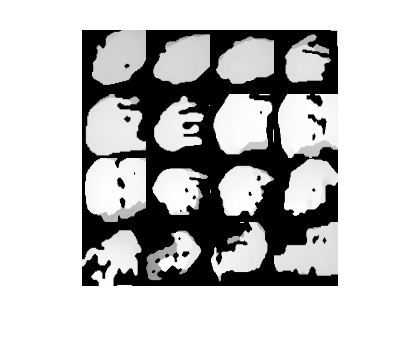
\includegraphics[width=0.45\textwidth]{figures/depth_hand.png}
  }
  \caption{$64\times64$ pixel raw image patches of hands.} \label{fig:hand}
\end{figure}

\begin{figure}[h]
\centering
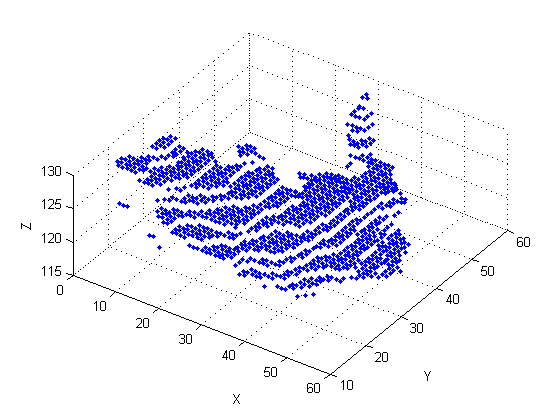
\includegraphics{figures/hand3d.png}
\caption{View of quantized depth data of a hand in 3D.}
\end{figure}

\section{Histogram of Oriented Gradients}
For each pixel, the magnitude of gradient is 
\begin{align*}
m = \sqrt{dx^2 + dy^2}
\end{align*}

If an image $I$ has dimensions $m\times n$, the size of the computed feature
vector $H$ is $(m/\text{cell\_size} - 2) \times (n/\text{cell\_size} - 2)
\times \text{num\_bin}$.

\begin{figure}[h]
  \centering
  \subfigure[Color] {
  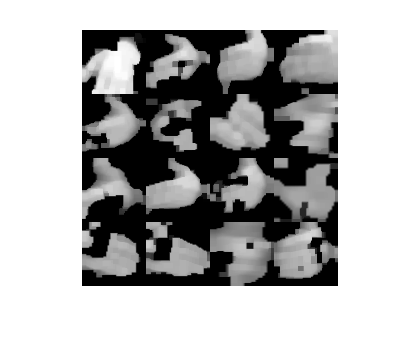
\includegraphics[width=0.45\textwidth]{figures/color_denoised_5.png} 
  }
  \subfigure[Depth] {
    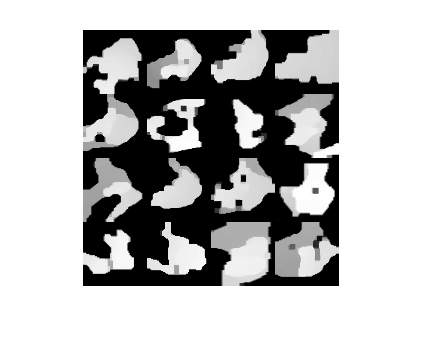
\includegraphics[width=0.45\textwidth]{figures/depth_denoised_5.png}
  }
  \subfigure[Color HOG] {
  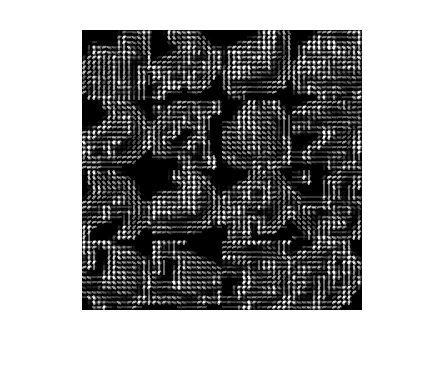
\includegraphics[width=0.45\textwidth]{figures/color_hog.png} }
  \subfigure[Depth HOG] {
    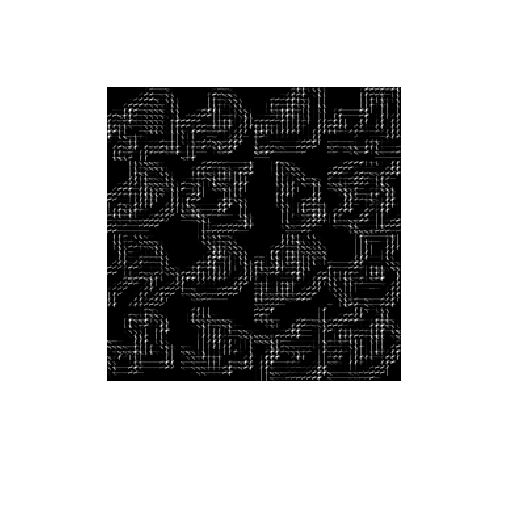
\includegraphics[trim={0cm 1.5cm 0cm 0cm},
  clip, width=0.5\textwidth]{figures/depth_hog.png}
  }
  \caption{$64\times64$ pixel image patches of hands.} \label{fig:hand}
\end{figure}

\section{Dictionary Learning}

\section{PCA and Sparse PCA}